\documentclass[12pt]{article}

\usepackage{fullpage}
\usepackage{fancybox}
\usepackage{graphicx}

\newcommand{\Max}{\textsf{\sc Maximum}}
\newcommand{\Insert}{\textsf{\sc Insert}}
\newcommand{\EM}{\textsf{\sc ExtractMax}}
\newcommand{\Combine}{\textsf{\sc Combine}}
\newcommand{\TP}{\textsf{\sc TylerPath}}
\newcommand{\DFS}{\textsf{\sc DFS}}
\newcommand{\EXPLORE}{\textsf{\sc Explore}}

\newcommand{\VISITED}{\mathord{\it visited}}
\newcommand{\TRUE}{\mathord{\it true}}
\newcommand{\FALSE}{\mathord{\it false}}
\newcommand{\CC}{\mathord{\it cc}}
\newcommand{\CCN}{\mathord{\it ccnumber}}

%%%%%%%%%%%%%% Capsule %%%%%%%%%%%%%%%%%%%%%%%%%%%%%%%%%%%%%%%%%%%
\newcommand{\capsule}[2]{\vspace{0.5em}
  \shadowbox{%
    \begin{minipage}{.90\linewidth}%
      \textbf{#1:}~#2%
    \end{minipage}}
  \vspace{0.5em} }
%%%%%%%%%%%%%%%%%%%%%%%%%%%%%%%%%%%%%%%%%%%%%%%%%%%%%%%%%%%%%%%%%%

\newcounter{ques}
\newenvironment{question}{\stepcounter{ques}{\noindent\bf Question \arabic{ques}:}}{\vspace{5mm}}
\newenvironment{solution}{{\noindent\bf Solution:}}{\vspace{5mm}}

\begin{document} 

\begin{center} \Large\bf
COMP 3804 --- Assignment 2 
\end{center} 

\noindent {\bf Due:} Thursday February 16, 23:59.

\vspace{0.5em}

\noindent {\bf Assignment Policy:}
\begin{itemize}
\item Your assignment must be submitted as one single PDF file through
      Brightspace.

\begin{center}
\hfill\shadowbox{
  \begin{minipage}{.90\linewidth}
    {\textsf{Use the following format to name your file:
        \[ {\tt LastName\_StudentId\_a2.pdf}
        \]
      }}
  \end{minipage}
}
\end{center}
\item {\bf Late assignments will not be accepted. I will not reply to
      emails of the type ``my internet connection broke down at
      23:57'' or ``my scanner stopped working at 23:58'', or
      ``my dog ate my laptop charger''.}
\item You are encouraged to collaborate on assignments, but at the level
      of discussion only. When writing your solutions, you must do so
      in your own words.
\item Past experience has shown conclusively that those who do not put
      adequate effort into the assignments do not learn the material and
      have a probability near 1 of doing poorly on the exams.
\item When writing your solutions, you must follow the guidelines below.
      \begin{itemize}
      \item You must justify your answers.
      \item The answers should be concise, clear and neat.
      \item When presenting proofs, every step should be justified.
      \end{itemize}
\end{itemize}

\newpage 

\begin{question}
Write your name and student number.
\end{question}

\begin{solution}
      Ryan Lo (101117765)
\end{solution}

\begin{question}
You are given $k$ sorted lists $L_1,L_2,\ldots,L_k$ of numbers. Let $n$ 
denote the total length of all these lists. 

Describe an algorithm that returns one list containing all these $n$ 
numbers in sorted order. The running time of your algorithm must be  
$O(n \log k)$.

Explain why your algorithm is correct and why the running time is 
$O(n \log k)$.

\noindent 
\emph{Hint:} If $k=2$, this should look familiar. 
\end{question}

\begin{solution}
      
      Algorithm:

      First start by creating a min-heap of size k.

      For each list $L_i$ we can insert the first element of $L_i$ into the min-heap.

      While the min-heap is not empty:

      We remove the smallest element from the min-heap

      Take that element and add it to the output list

      Finally return the output list

      Correctness:

      For k = 2, the algorithm is just a standard merge sort, which is proved to be correct.
      Assume now that in the algorithm we have is correct for k-1 lists. We no consider having k lists,
      so $L_1,L_2,\ldots,L_k$. We can now pair up each lists into k/2 pairs and merge them together
      into a single sorted list using the algorithm for two lists as stated above which is correct.
      If k is even then the lists are paired evenly and works out perfectly, if k is odd
      then we have a left over list which we can just merge with the main list.
      After everything is finished we get a single sorted list that contains all n elements
      from the k amount of lists and therefore is correct.
\end{solution}

\begin{question}
{\bf This is a long question. Don't be intimidated! As always, for 
each part in this question, you must justify your answer.} 

Professor Justin Bieber needs a data structure that maintains a collection 
$A,B,C,\ldots$ of sets under the following operations:
\begin{enumerate} 
\item $\Max(X)$: return the largest element in the set $X$. 
\item $\Insert(X,y)$: add the number $y$ to the set $X$. 
\item $\EM(X)$: delete and return the largest element in the set $X$. 
\item $\Combine(X,Y)$: take the union $X \cup Y$ of the sets $X$ and 
      $Y$, and call the resulting set~$X$.  
\end{enumerate} 
Professor Bieber knows how to support the first three operations: 
Store each set $X$ in a max-heap. The fourth operation seems to be 
more problematic, because we have to take two max-heaps and combine 
them into one max-heap. 

To support all four operations, Professor Bieber has invented the 
following sequence $B_0,B_1,B_2,\ldots$ of trees, which are now 
universally known as \emph{Bieber trees}:     
\begin{enumerate} 
\item $B_0$ is a tree with one node. 
\item For each $i \geq 1$, the tree $B_i$ is obtained as follows: 
Take two copies of $B_{i-1}$ and make the root of one copy a child of the 
root of the other copy. 
\end{enumerate} 

\begin{center}
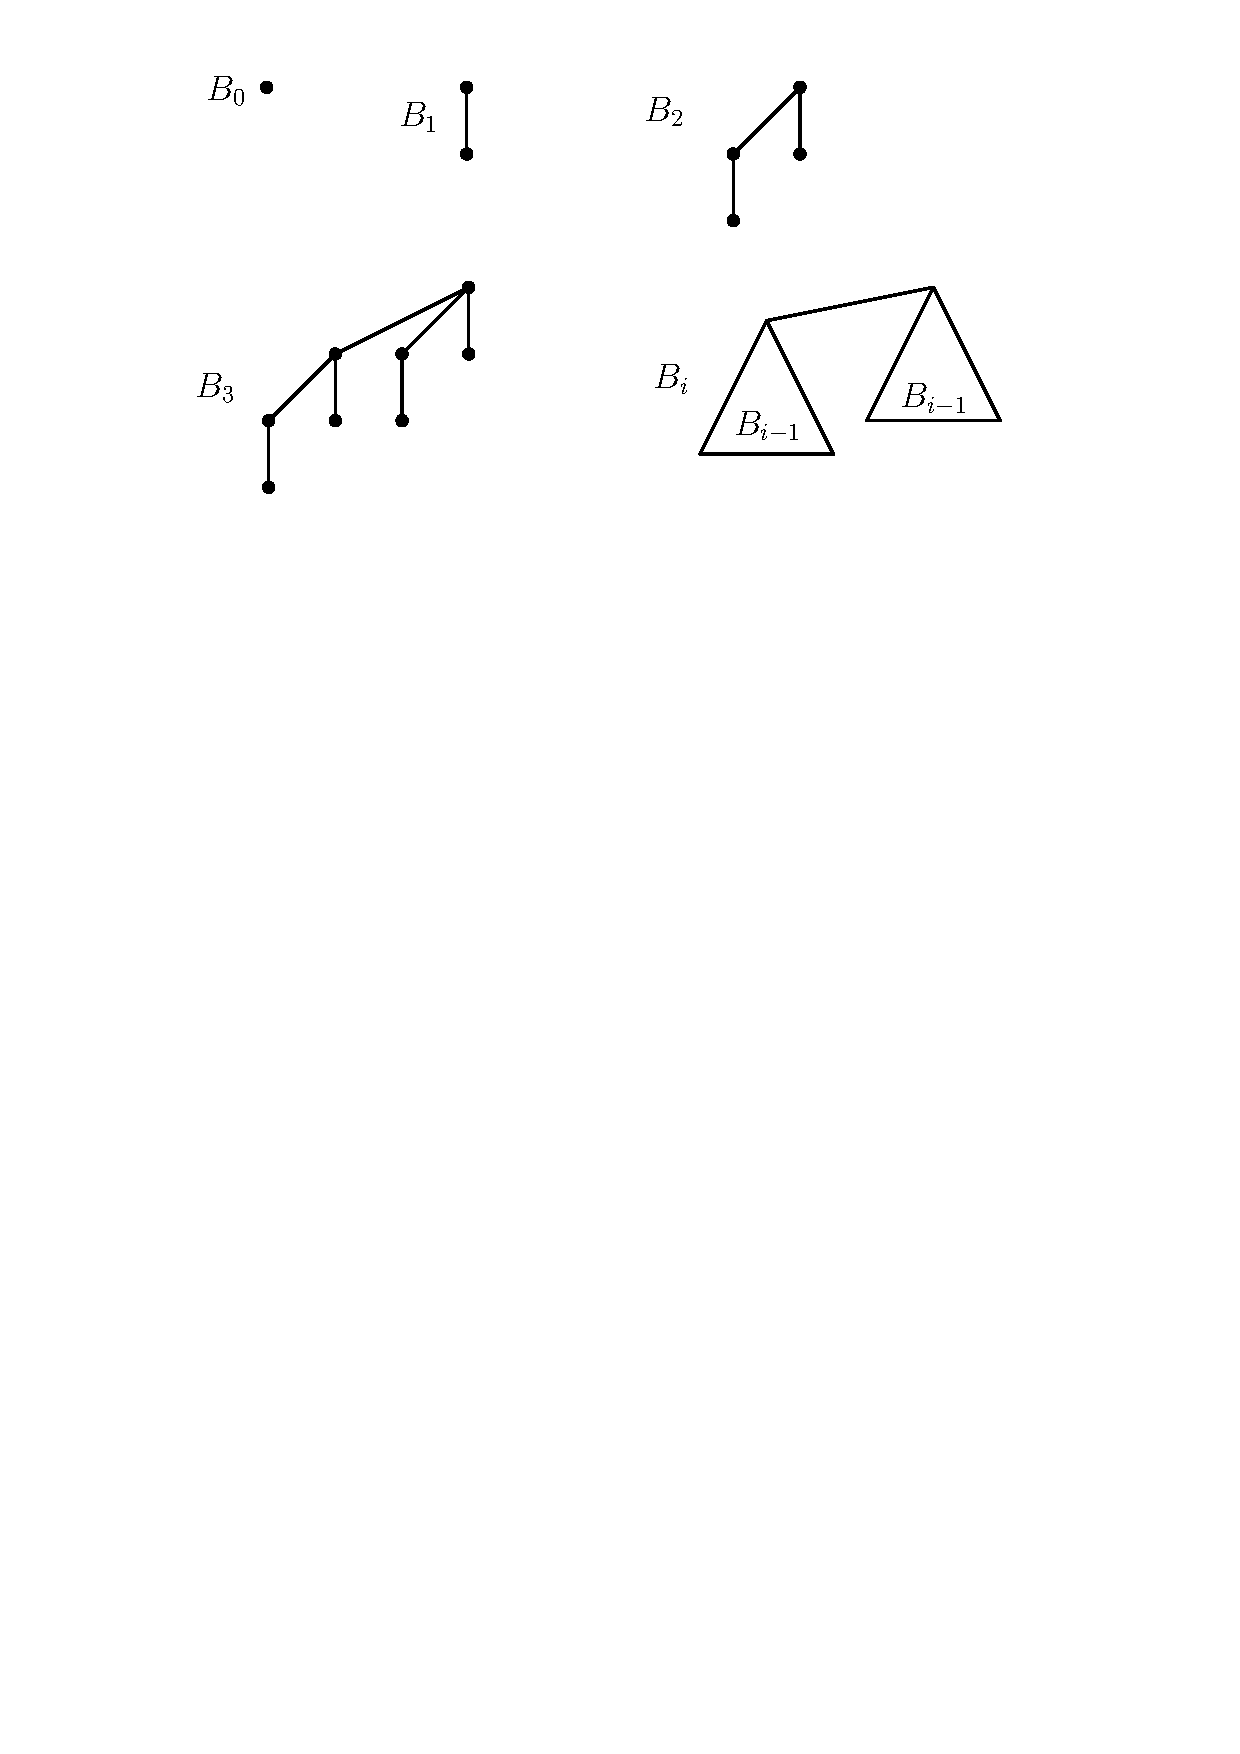
\includegraphics[scale=0.60]{Biebertrees}
\end{center}

\noindent 
{\bf Question 3.1:} Let $i \geq 0$. How many nodes does the tree $B_i$ 
have? 

\vspace{0.5em} 

\begin{solution}
      
      The tree is doubling in nodes every time. Therefore the tree $B_i$ has $2^i$ nodes.
\end{solution}

\vspace{0.5em} 

\noindent 
{\bf Question 3.2:} Let $i \geq 0$. What is the height of the tree $B_i$? 

\vspace{0.5em} 

\begin{solution}
      
      The height of the tree increases every time. Therefore the height of the tree $B_i$ is $i+1$.
\end{solution}

\vspace{0.5em} 

\noindent 
{\bf Question 3.3:} Let $i \geq 1$. Prove that the subtrees of the root 
of $B_i$ are the Bieber trees $B_0,B_1,\ldots,B_{i-1}$. 

\vspace{0.5em} 

\begin{solution}
      
      We will prove this by induction that the subtrees of the root of $B_i$ are Bieber trees.

      Base Case: 

      When i = 0, the root of $B_0$ is just a single node. The only subtree of the root is the root itself,
      so the subtree is the Bieber tree which is $B_0$.

      Inductive Case:

      We assume that the subtrees of the root of $B_i$ are Bieber trees $B_0,B_1,\ldots,B_{i-1}$.
      Now we want to show the the subtress of the root of $B_i+1$ are Bieber tress $B_0,B_1,\ldots,B_{i}$.
      From the definition of a Bieber tree, the Bieber tree $B_i+1$ is formed by taking two copies of
      $B_i$ and then attaching the root of one to the root of the other. Therefore the tree contains 
      a subtree that is a Bieber tree. The Bieber tree $B_i+1$ contains 2 instances of the Bieber subtree
      $B_i$, one rooted at the root and the second one which is the root itself. 
      The subtrees $B_i$ rooted at the root of the $B_i+1$ tree are copies of $B_i$
      which by the inductive hypothesis, they are the Bieber trees $B_0,B_1,\ldots,B_{i-1}$.

\end{solution}

\vspace{0.5em} 

Let $X$ be a set of $n$ numbers, assume that $n \geq 1$, and let 
\[ n = (b_m,b_{m-1},\ldots,b_1,b_0) 
\]
be the binary representation of $n$. Note that $b_m = 1$ and 
\[ n = \sum_{i=0}^m b_i \cdot 2^i . 
\] 
The 
\emph{Bieber max-heap} for the set $X$ is obtained as follows: 
\begin{enumerate} 
\item Partition the set $X$, arbitrarily, into subsets such that 
for each $i$ for which $b_i = 1$, there is exactly one subset 
of size $2^i$. 

For example, if $n = 11 = 2^3 + 2^1 + 2^0$, the set $X$ is partitioned 
into three subsets: one of size $2^3$, one of size $2^1$, and one of size 
$2^0$. 
\item Each subset of size $2^i$ is stored in a Bieber tree $B_i$. 
Each node in $B_i$ stores one element of the subset. Each node in $B_i$ 
has pointers to its parent and all its children. There is a pointer 
to the root of $B_i$.   
\item Each Bieber tree has the property that the value stored at a 
node is larger than the values stored at any of its children. 
\item The roots of all these Bieber trees are connected using a 
doubly-linked list. 
\end{enumerate} 
The figure below gives an example when $n=11$. 

\begin{center}
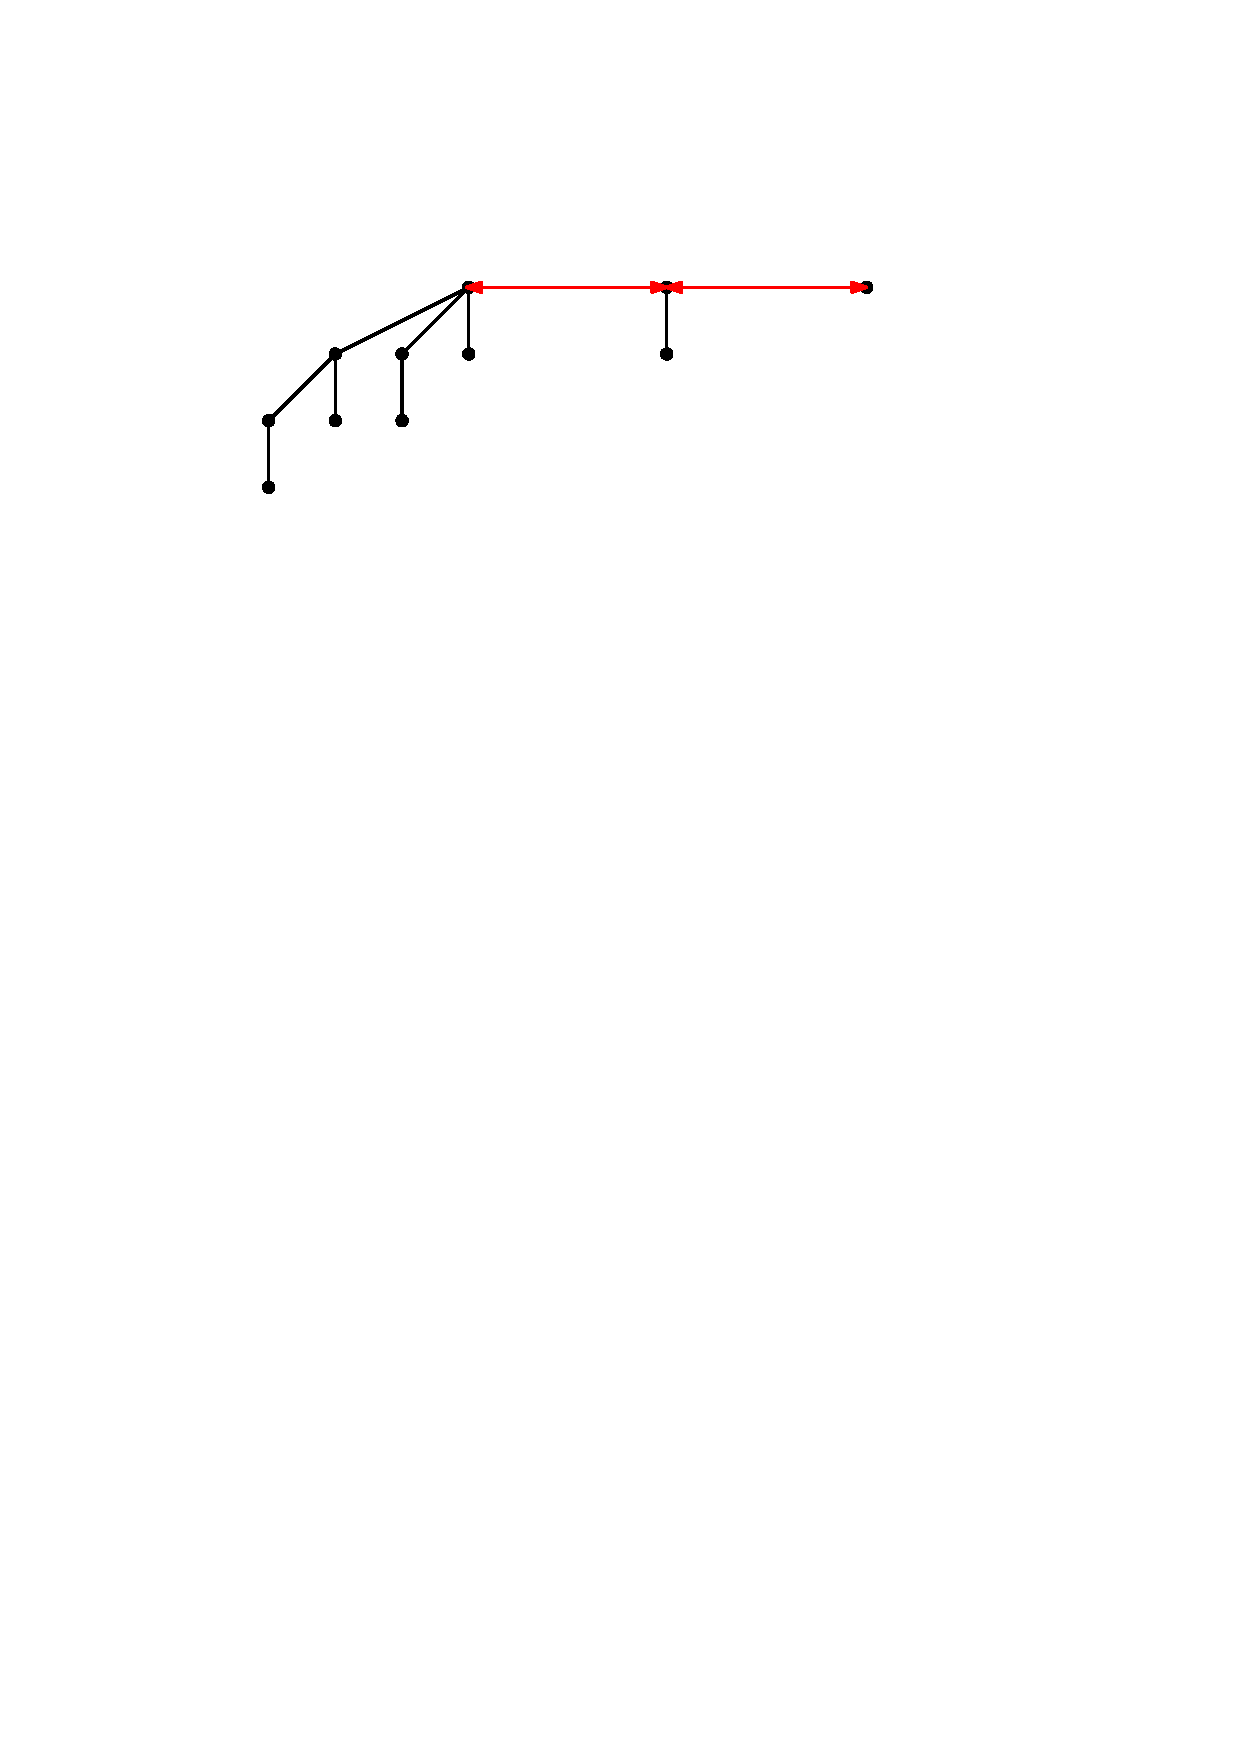
\includegraphics[scale=0.60]{Bieberheap}
\end{center}

\noindent 
{\bf Question 3.4:} Let $X$ be a non-empty set of numbers, and assume 
that this set is stored in a Bieber max-heap. Describe an algorithm 
that implements the operation $\Max(X)$ in $O(\log |X|)$ time. 

\vspace{0.5em} 

\begin{solution}
      
      Algorithm:

      Start by following through the doubly linked-list to find the maximum element.
      Then compare the current maximum value with each root. Update the maximum if the 
      value is larger. Continue traversing till the very end. Return the maximum value found.
      It will take $O(log |X|)$ to traverse through the Bieber tree. 

\end{solution}

\vspace{0.5em} 

\noindent 
{\bf Question 3.5:} Let $X$ and $Y$ be two sets of numbers, and assume 
that both sets have the same size $2^i$. A Bieber max-heap 
for $X$ consists of one single Bieber tree $B_i$. Similarly, a 
Bieber max-heap for $Y$ consists of one single Bieber tree $B_i$. 
Describe an algorithm that implements the operation 
$\Combine(X,Y)$ in $O(1)$ time. 

\vspace{0.5em} 

\begin{solution}
      
      To combine two Bieber max-heaps we can make the root of the Bieber tree for Y
      a child of the root of the Bieber tree for X. Since each of the values is stored
      at a node that is larger than the values stored at any of its children it follows
      the Bieber max-heap.

      Algorithm:

      First we attach the root of the Bieber tree for Y to the root of the Bieber tree for X

      Next we update the connects of the roots for X and Y

      This operation would take constant time.

\end{solution}

\vspace{0.5em} 

\noindent 
{\bf Question 3.6:} Let $X$ and $Y$ be two non-empty sets of numbers, and  
assume that $X$ is stored in a Bieber max-heap and $Y$ is stored in 
a Bieber max-heap. Describe an algorithm that implements the operation 
$\Combine(X,Y)$ in $O( \log |X| + \log |Y| )$ time. 

\noindent 
\emph{Hint:} This operation computes one Bieber max-heap storing the 
union $X \cup Y$. If you take the sum of two integers, both given 
in binary, then you go through the bits from right to left and keep 
track of a carry bit.   

\vspace{0.5em} 

\begin{solution}
      
      Algorithm:

      First, we want to merge X and Y using the union of both of them
      X $\cup$ Y and we will label this new set Z.
      Next we need to create a new Bieber tree for the set Z, we do this by
      spliting the $B_i-1$ into 2 copies until Z becomes a Bieber tree.
      Then we update the doubly linked list of the Bieber trees to add in the 
      new root
      Finally, we do a Bieber max-heapify on the Bieber tree to keep the Bieber
      max heap property.

      First step takes $O(|X| + |Y|)$, second step takes $O(|Z|)$ time to get the Bieber tree
      , third step takes $O(1)$ time because it's just linked list pointer upates
      and last step takes $O(|Z|)$ time to heapify the tree.

      The total time complexity of the whole operation is $O(log |X| + log |Y|)$ time.

\end{solution}

\vspace{0.5em} 

\noindent 
{\bf Question 3.7:} Let $X$ be a non-empty set of numbers, and assume 
that this set is stored in a Bieber max-heap. Describe an algorithm
that implements the operation $\Insert(X,y)$ in $O(\log |X|)$ time. 

Note that this operation computes a Bieber max-heap for the set 
$X \cup \{y\}$. 

\vspace{0.5em} 

\begin{solution}
      
      Algorithm:

      If y is greater than the value that is in the root of the Bieber tree
      then create a new Bieber tree $B_i+1$ with y as the root and make the new
      tree a child of of it. Otherwise, make a new node with y and add it to the
      existing Bieber tree.
      If we were to traverse through, the worst case would be $O(log |X|)$ time.

\end{solution}

\vspace{0.5em} 

\noindent 
{\bf Question 3.8:} Let $X$ be a non-empty set of numbers, and assume 
that this set is stored in a Bieber max-heap. Describe an algorithm
that implements the operation $\EM(X)$ in $O(\log |X|)$ time. 

Note that this operation computes a Bieber max-heap for the set 
$X \setminus \{y\}$, where $y$ is the largest number in $X$. 

\vspace{0.5em} 

\begin{solution}
      
      Algorithm:

      To start we extract the maximum value from the root of the Bieber tree.
      Next we have to rebuild the remaining Bieber trees. To do this we have to
      repeatly merge the Bieber trees together until it becomes one connected tree.
      The time complexity for the whole algorithm takes $O(log |X|)$ time to perform
      , there is going to be at most log $|X|$ levels.

\end{solution}

\vspace{0.5em} 

\noindent 
{\bf Question 3.9:} Let $X$ be a non-empty set of numbers, and assume 
that this set is stored in a Bieber max-heap. How would you extend 
this data structure such that the operation $\Max(X)$ only takes 
$O(1)$ time, whereas the running times for the other operations 
$\Combine$, $\Insert$, and $\EM$ remain as above? 
\end{question}

\vspace{0.5em} 

\begin{solution}
      
      An easy and simple way to extend this data structure such that the operation
      of MAXIMUM(X) only takes O(1) time is to add and maintain an extra pointer to the maximum
      element in the heap. Whenever we run combine the we can just compare the two maximums
      between the two heaps and update the pointer to the new maximum. Running insert we just
      compare the newly inserted element with the current maximum and update if needed.
      For extract maximum, we can just return the maximum that the pointer is pointing to
      then remove it from the heap. Finding the new maximum element and assigning the pointer to it
      will take only $O(log |X|)$ when does not hinder the performance. With that the 
      new MAXIMUM(X) will be O(1) with changing the runtime of the other operations.

\end{solution}

\begin{question}
Consider the following undirected graph:

\begin{center}
     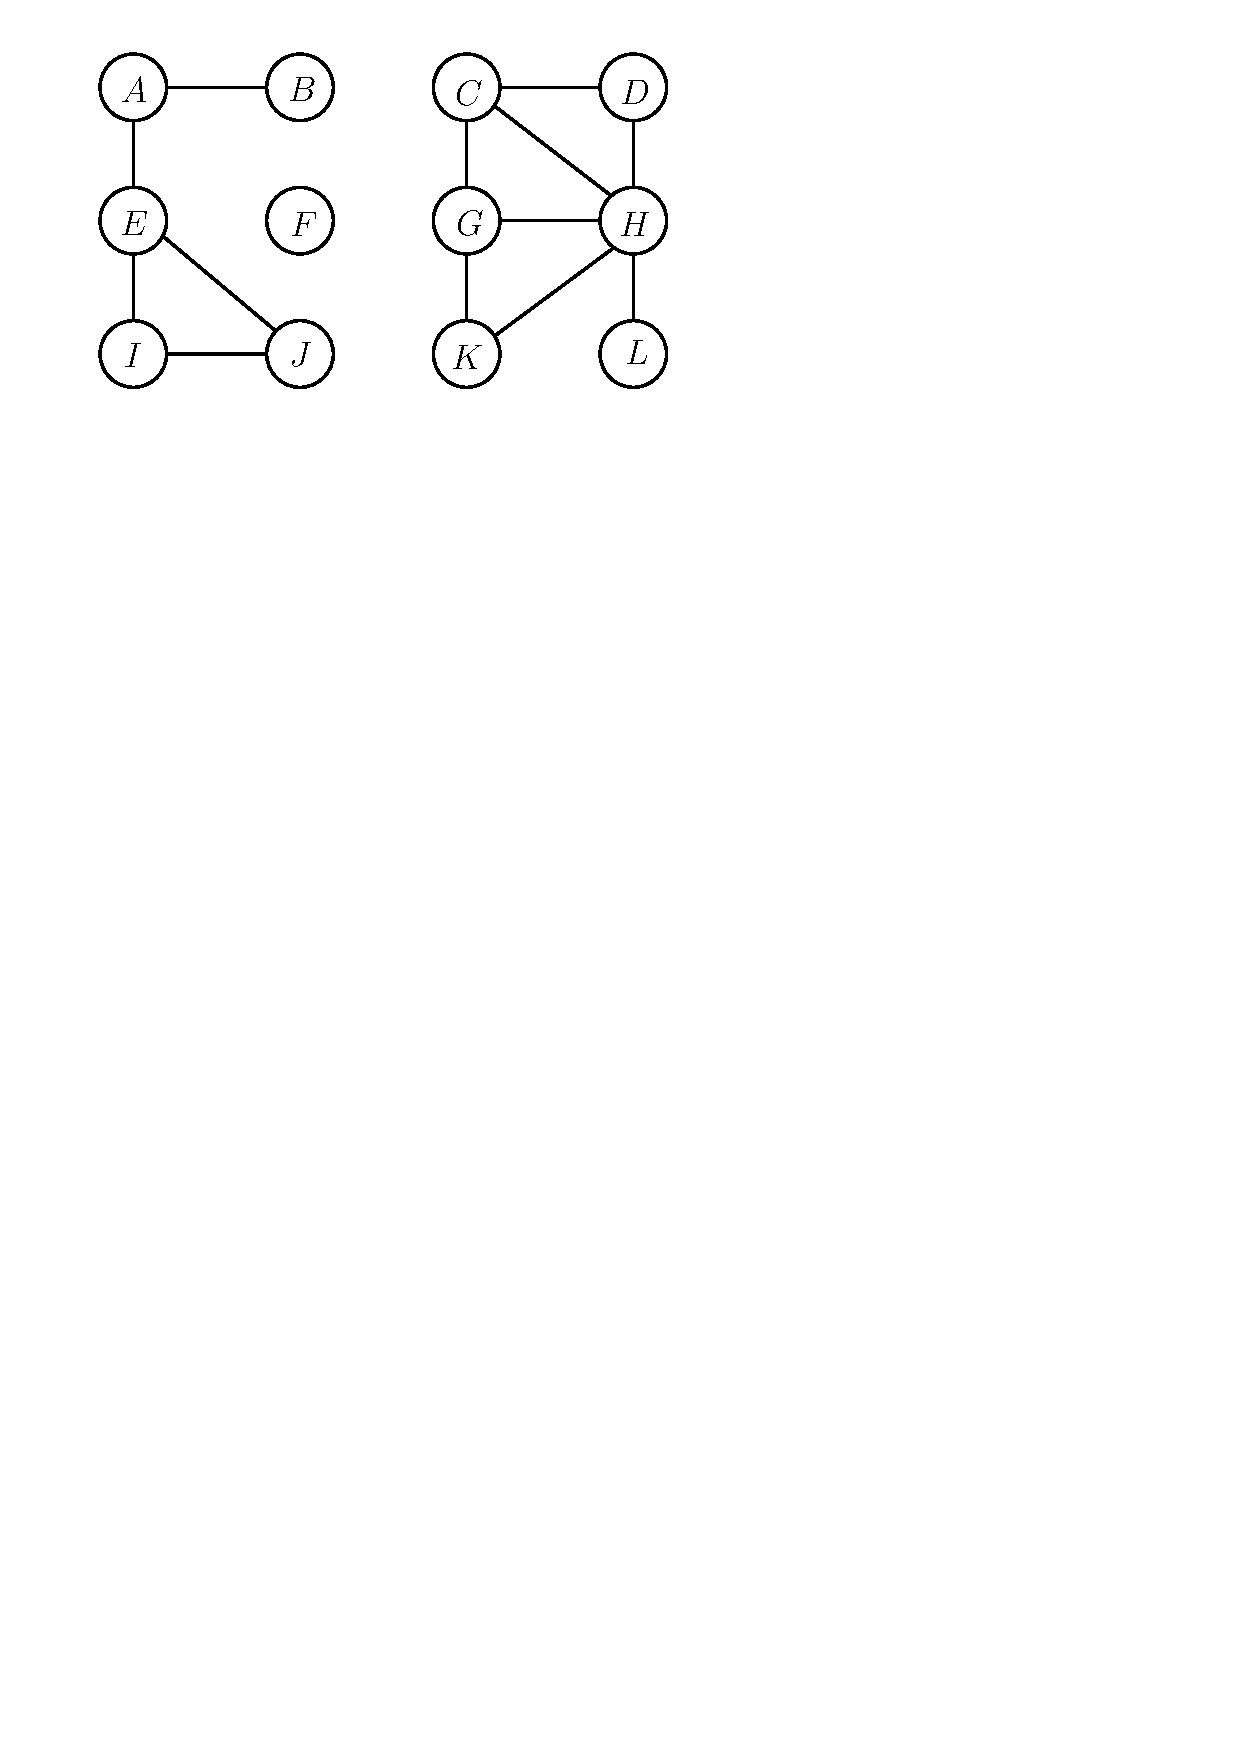
\includegraphics[scale=0.7]{graph}
\end{center}

Draw the $\DFS$-forest obtained by running algorithm $\DFS$ on 
this graph. The pseudocode is given at the end of this assignment. 
Algorithm $\DFS$ uses algorithm $\EXPLORE$ as a subroutine; the 
pseudocode for this subroutine is also given at the end of this 
assignment.

In the forest, draw each tree edge as a solid edge, and draw each back 
edge as a dotted edge. 

Whenever there is a choice of vertices, pick the one that is 
alphabetically last.
\end{question}

\vspace{0.5em} 

\begin{solution}
      
      Reverse alphabetical order:

      Assuming it is stored as: [L, K, J, I, H, G, F, E, D, C, B, A]

      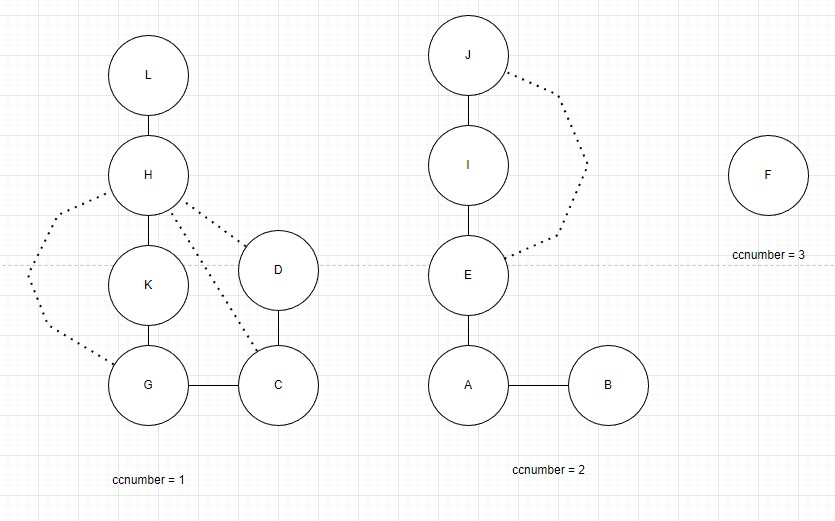
\includegraphics[scale=0.87]{DFSreverse.jpg}

\end{solution}

\newpage 

\begin{question} 
Tyler is not only your friendly TA, he is also the inventor of 
Tyler paths and Tyler cycles in graphs: 
A \emph{Tyler path} in an undirected graph is a path that 
contains every vertex exactly once. In the figure below, you see a Tyler 
path in red. A \emph{Tyler cycle} is a cycle that contains every vertex 
exactly once. In the figure below, if you add the black edge $\{s,t\}$ 
to the red Tyler path, then you obtain a Tyler cycle.    

\begin{center}
     \includegraphics[scale=0.7]{TylerPath}
\end{center}

If $G=(V,E)$ is an undirected graph, then the graph $G^3$ is defined 
as follows: 
\begin{enumerate} 
\item The vertex set of $G^3$ is equal to $V$. 
\item For any two distinct vertices $u$ and $v$ in $V$, $\{u,v\}$ is an 
edge in $G^3$ if and only if there is a path in $G$ between $u$ and $v$ 
consisting of at most three edges. 
\end{enumerate} 

\noindent 
{\bf Question 5.1:} 
Describe a \emph{recursive} algorithm $\TP$ that has the following 
specification:

\capsule{Algorithm $\TP(T,u,v)$}{

{\bf Input:} A tree $T$ with at least two vertices; two distinct 
vertices $u$ and $v$ in $T$ such that $\{u,v\}$ is an edge in $T$. 

{\bf Output:} A Tyler path in $T^3$ that starts at vertex $u$ and ends 
at vertex $v$. 
}

\noindent 
\emph{Hint:} You do not have to analyze the running time. 
The base case is easy. Now assume that $T$ has at least 
three vertices. If you remove the edge $\{u,v\}$ from $T$, then you 
obtain two trees $T_u$ (containing $u$) and $T_v$ (containing $v$). 
\begin{enumerate} 
\item One of these two trees, say, $T_u$, may consist of the single 
vertex $u$. How does your recursive algorithm proceed?    

\vspace{0.5em} 

\begin{solution}
      
      The case where $T_u$ consist of a single vertex $u$, in this case the edge ${u,v}$
      is the Tyler path from u to v. The other case where the edge ${u,v}$ is in the
      other tree, the Tyler path from u to v is the path that consists of u, the edge
      ${u,v}$ and a Tyler path from v to a node in $T_v$.

\end{solution}

\item If each of $T_u$ and $T_v$ has at least two vertices, how 
does your recursive algorithm proceed?    
\end{enumerate} 

\vspace{0.5em} 

\begin{solution}
      
      If $T_u$ and $T_v$ both has at least 2 vertices, we can first take $T_u$ and find the
      Tyler path from u to another vertex in $T_u$ which we can call x. Now we can take
      $T_v$ and then find the Tyler path from v to another vertex in $T_v$ which we can 
      label as y. Now we can take both the Tyler paths in $T_u$ and $T_v$ which we just found
      and insert an edge from x to y we can get a Tyler path from $T_u$ to $T_v$.

\end{solution}

\vspace{0.5em} 

\noindent 
{\bf Question 5.2:} 
Prove the following lemma: 

\vspace{0.5em} 

\noindent 
{\bf Tuttle's Lemma:} For every tree $T$ that has at least three vertices, 
the graph $T^3$ contains a Tyler cycle.   

\vspace{0.5em} 

\begin{solution}
      
      Base Case: If T has 3 vertices, the Tyler path is the path that just contains all
      three vertices. 

      Inductive Case: We now assume that T has at least four vertices. Say we have two trees
      $T_u$ and $T_v$, and we remove the edge ${u, v}$, and we have a vertex x that is
      connected to both u and v. We can add the path from v to the vertex x. 
      With that the graph T still contains a path from v to x and a path from x to u.
      It connects all the vertices creating a Tyler cycle. Therefore it contains
      a Tyler cycle. 

\end{solution}

\vspace{0.5em} 

\noindent 
{\bf Question 5.3:} 
Prove the following theorem: 

\vspace{0.5em} 

\noindent 
{\bf Tuttle's Theorem:} For every connected undirected graph $G$ that 
has at least three vertices, the graph $G^3$ contains a Tyler cycle.   
\end{question}

\vspace{0.5em} 

\begin{solution}
      
      Base Case: If T has 3 vertices, the Tyler cycle is the cycle that just contains all
      three vertices. 

      Inductive Case: Assume that the graph G has at least four vertices. Since the
      graph is connected there is a path P where it starts at a vertex u and goes
      around and visits all vertices in the connected part then returns back to the
      vertex u. The Tyler cycle still contains all vertices in the cycle so therefore
      it is still a Tyler cycle.

\end{solution}

\newpage

\begin{quote}
\begin{tabbing}
{\bf Algorithm} $\DFS(G)$: \\
{\bf for each} vertex $u$ \\
{\bf do} $\VISITED(u) = \FALSE$ \\
{\bf endfor}; \\
$\CC = 0$; \\ 
{\bf for each} vertex $v$ \\
{\bf do} \= {\bf if} $\VISITED(v) = \FALSE$ \\
         \> {\bf then} \= $\CC = \CC + 1$ \\ 
         \>            \> $\EXPLORE(v)$  \\
         \> {\bf endif} \\
{\bf endfor} \\
\end{tabbing}
\end{quote}

\begin{quote}
\begin{tabbing}
{\bf Algorithm} $\EXPLORE(v)$: \\
$\VISITED(v) = \TRUE$; \\
$\CCN(v) = \CC$; \\ 
{\bf for each} edge $\{v,u\}$ \\
{\bf do} \= {\bf if} $\VISITED(u) = \FALSE$ \\
         \> {\bf then} \= $\EXPLORE(u)$ \\
         \> {\bf endif} \\
{\bf endfor} \\
\end{tabbing}
\end{quote}

\end{document} 